    \subsection{Целый базис для расширения полного поля}

    
	Пусть $(K, \v)$~--- полное нормированное поле, $L/K$~--- конечное расширение (на которое мы можем продолжить нормирование), а 
	\[
	 	\cO_{L} = \{ x \in K^* \ \vert \ \v(x) > 0 \}, \quad \cO_{L} = \{ x \in L^{*} \ \vert \ w(x) > 0 \}, \quad w \mid \v.
	 \] 

	 Пусть $\Bbbk = \cO_{L}/\fp_{K}, \ \ell = \cO_{L}/\fp_{L}$~--- поля вычетов, а  
	 \[
	 	f\lr*{L/K} = [\ell : \Bbbk], \quad e\lr*{L/K} = w(\pi), \text{ где } \pi_{K} \in \cO_{K}, \ \v(\pi) = 1, \quad w(\pi_{L}) = 1.
	 \]

	 В частности, если расширение сепарабельно, то $ef = n$. 

	 \begin{statement} 
	 	$\cO_{L}$~--- свободный $\cO_{K}$-модуль ранга $n$.
	 \end{statement}
	 \begin{proof}
	 Пусть $\omega_1, \ldots, \omega_{f} \in \cO_{L}$~--- такие, что $\overline{\omega_1}, \ldots, \overline{\omega_{f}}$~--- базис $\ell/\Bbbk$. Рассмотрим набор 
	 \[
	 	\{ \omega_i \pi_{L}^{j} \}_{1 \le i \le f,\  0 \le j \le e - 1}
	 \]
	 и проверим, что он образует базис $\cO_{L}$ над $\cO_{K}$. Проверим сначала линейную независимость. Рассмотрим линейную комбинацию: 
	 \[
	 	\sum_{i, j} a_{i j} \omega_{i} \pi_{L}^{j} = 0 \Leftrightarrow  \sum_{j} \lr*{\sum_{i} a_{i j} \omega_{i} } \pi_{L}^{j} = 0. 
	 \]
	 Пусть $P_{1} = \{ 0 \le j \le e - 1 \ \vert \ \forall i \  \v(a_{i j}) \ge 1 \}$, а $P_{2} = \{ 0 \le j \le e - 1 \ \vert \ \exists i \colon \v(a_{i j}) = 0\}$. Ясно, что они дополняют друг друга, то есть $P_1 \sqcup P_2 = \{ 0, 1, \ldots, e - 1 \}$.  Заметим, что для $j \in P_1$
	 \[
	 	w\lr*{\lr*{\sum_{i} a_{i j} \omega_{i} } \pi_{L}^{j}} \ge e \implies w\lr*{\sum_{j \in P_1} \lr*{\sum_{i} a_{i j} \omega_{i} } \pi_{L}^{j}} \ge e. 
	 \]
	 Если $j \in P_2$, то перейдём к образу в поле вычетов: 
	 \[
	 	\sum_{} \overline{a_{i j}} \overline{\omega_i} \neq 0 \in \ell,
	 \]
	 так как $\{ \overline{\omega_i}\}$~--- базис $\ell/\Bbbk$, то есть элемент не лежит в идеале нормирования. Тогда 
	 \[
	 	w\lr*{\sum_{i} a_{i j} \omega_{i}} = 0 \implies w\lr*{\lr*{\sum_{i} a_{i j} \omega_{i}} \pi_{L}^{j}} = j.
	 \]
	 Тогда, суммируя мы получим, что 
	 \[
	 	\sum_{j \in P_2} \lr*{\sum_{j \in P_2} a_{i j} \omega_{i}} \pi_{L}^{j} = \min_{j \in P_2}{j} \le e - 1. 
	 \]

	 Так мы приходим к противоречию, так как 
	 \[
	 	\sum_{j \in P_1} \lr*{\sum_{i} a_{i j} \omega_{i} } \pi_{L}^{j}  = - \sum_{j \in P_2} \lr*{\sum_{i} a_{i j} \omega_{i} } \pi_{L}^{j}.
	 \]
	 Если $P_2 \neq \varnothing$, то мы пришли к противоречию, так как нормирование левой части $\ge e$, а номрирование правой части $\le e - 1$.

	 Если же $P_2 = \varnothing,$ все $a_{i j} \divby \pi_{K}$. Тогда мы можем делить коэффициенты на $\pi_{K}$ до тех пор, пока хотя бы один из коэффициентов не будет не делиться на $\pi_K$. Если коэффициенты ненулевые, то в какой-то момент мы таким образом добьемся, что $P_2 \neq \varnothing$, что нам и нужно. 

	 Покажем теперь, что это система образующих. Возьмём $x_0 = x \in \cO_{L}$, рассмотрим $\overline{x} \in \ell$ и разложим по базису $\ell/\Bbbk$:
	 \[
	 	\overline{x} = \sum_{i = 1}^{f} \overline{a_{i}} \cdot \overline{\omega_i} \rightsquigarrow x_0 = a_{0 1} \omega_1 + \ldots + a_{0 f} \omega_f + \pi_L x_1.
	 \]
	 Проделаем аналогичную процедуру для элемента $x_1 \in \cO_{L}$: 
	 \[
	 	\begin{cases} 
	 	x_0 = a_{0 1} \omega_1 + \ldots + a_{0 f} \omega_f + \pi_L x_1 \\
	 	x_1 = a_{1 1} \omega_1 + \ldots + a_{1 f} \omega_f + \pi_L x_1 \\ 
	 	\vdots \\ 
	 	x_{e - 1} = a_{e - 1, 1} \omega_{1} + \ldots + a_{e - 1, f} \omega_{f} + \pi_{L} x_{e}.
	 	 \end{cases}
	 \]
	 Домножим второе уравнение на $\pi_{L}$, третье на $\pi_{L^2}$ и так далее, и сложим. Тогда мы получим: 
	 \[
	 	x = \sum_{1 \le i \le f, \ 0 \le j e - 1 } \alpha_{i j}^{(0)} \omega_i \pi_{L}^{j} + \pi_{L}^{e} y 
	 \]
	 Так как $\pi_K = \pi_L^{e} t$, где $t$ обратим, мы можем переписать эту сумму вот в таком виде: 
	 \[
	 	x = \sum_{1 \le i \le f, \ 0 \le j e - 1 } \alpha_{i j}^{(0)} \omega_i \pi_{L}^{j} + \pi_{K} \widetilde{x_1}, \quad \widetilde{x_1} \in \cO_{L}.
	 \]
	 Для $\widetilde{x_1}$ мы можем записать аналогичное равенство: 
	 \[
	 	\begin{cases} \widetilde{x_1} = \sum_{1 \le i \le f, \ 0 \le j e - 1 } \alpha_{i j}^{(1)} \omega_i \pi_{L}^{j} + \pi_{K} \widetilde{x_2}, \quad \widetilde{x_2} \in \cO_{L} \\
		\widetilde{x_2} = \sum_{1 \le i \le f, \ 0 \le j e - 1 } \alpha_{i j}^{(2)} \omega_i \pi_{L}^{j} + \pi_{K} \widetilde{x_3}, \quad \widetilde{x_3} \in \cO_{L} \\ 
		\vdots
	 	\end{cases}
	 \]
	 Домножим первое равенство на $\pi_k$, второе на $\pi_K^2$  сложим (тут строчек бесконечное число, но так как общий член стремится у нулю, всё в порядке). Тогда мы получим 
	 \[
	 	x = \sum \alpha_{i j} \omega_i \pi_{L}^j, \quad \alpha_{i j} \in \cO_{K},
	 \]
	 что и требовалось. 
	 \end{proof}

	 Рассмотрим теперь башню полей $E/L/K$. Тогда нетрудно заметить, что 
	 \[
	 	e\lr*{E/K} = e\lr*{E/L} \cdot e\lr*{L/K}, \quad f\lr*{E/K} = f\lr*{E/L} \cdot f\lr*{L/K}.
	 \]
	 Пусть $\overline{E},\overline{K}, \overline{L}$. Тогда второе утверждение~--- просто лемма о башне, а первое утверждение следует из того, что 
	 \[
	 	\pi_{K} = \pi_{L}^{e\lr*{L/K}} \cdot u, \ u \in \cO_{L}^{*}, \quad \pi_{L} = \pi_{E}^{e\lr*{E/L}} v, \quad v \in E^{*} \rightsquigarrow \pi_{K} = \pi_{E}^{e\lr*{E/L} \cdot e\lr*{L/K}} \cdot s, \quad s \in E^{*}.
	 \]

	 Эти равенства оказываются весьма удобными, когда необходимо вычислять индексы ветвления и степени инерции. 

	 С этого момента мы будем повсеместно полагать поле $K$ полным относительно нормирования $\v$. 

	 \subsection{Неравзветвлённые и вполне разветвлённые расширения}

	 Обычно выделяют два типа расширений такого поля $K$:

	 \begin{definition} 
	 	Пусть $K$~--- полное поле, тогда конечное расширение $L/K$ называется \emph{неравзетвлённым}, если $e(L/K) = 1$, а $\ell/\Bbbk$~--- сепарабельно. 

	 	Оно же называется \emph{вполне разветвлённым}, если $f\lr*{L/K} = 1$. 
	 \end{definition}

	 \begin{remark}
	 	В случае, когда поле вычетов конечно (а это как раз интересный нам случай), сепарабельность есть автоматически. 

	 	Отметим также, что в случае вполне разветвленного расширения мы не требуем сепарабельности. 
	 \end{remark}

	 \begin{example}
	 	Например, если $L = K(\theta)$, где 
	 	\[
	 		\theta^n + a_{n - 1}\theta^{n - 1} + \ldots + a_1 \theta + a_0 = 0
	 	\]
	 	и, минимальный многочлен $\theta$ Эйзенштейнов, то есть, $\v(a_i) \ge 1, \ \v(a_0) = 1$. Тогда $L/K$~--- вполне равзетвлённое расширение. 

	 	Кроме того, верно и обратное: любое равзетвлённое расширение полного поля $K$ получается присоединением корня многочлена Эйзенштейна. 
	 \end{example}

	 \begin{example}
	 	Рассмотрим над $\Q_{p}$ многочлен $x^2 - pu, \ u \equiv 1 \pmod{p}, \ u \neq 1$. Тогда, так как $u \in \Q_{p}^{*2}$, мы всегда получим расширение $\Q_{p}\lr*{\sqrt{p}}$. Значит, различные многочлены Эйзенштейна могут давать одно и то же расширение.  

	 	С другой стороны, если $x^2 - p \varepsilon	$, где $\varepsilon \notin \Q_{p}^{*2}$, мы получаем вполне разветвлеённое расширение $\Q_{p}\lr*{\sqrt{p \varepsilon}}$. 

	 	А вот расширение $\Q_{p}\lr*{\sqrt{\varepsilon}}$ будет неразветвлённым.

	 	Оказывается, если поле вычетов конечно (как в этом случае), то существует ровно одно неравзетвлённое расширение заданной степени. 
	 \end{example}

	 \begin{example}
	 	Нетрудно придумать пример, когда поле вычетов будет алгебраически замкнутым. Пусть $\Bbbk$~--- алгебраически замкнутое, рассмотрим поле $\Bbbk((t))$. Оно является полным относительно нормирования 
	 	\[
	 		\v(f) = n, \quad f = t^n (a_0 + a_1 t + \ldots ).
	 	\]
	 	В данном случае $\cO_{K} = \Bbbk[[t]]$, а $\fm_{\v} = (t)$, откуда $\fm_{\v} = \Bbbk$. 
	 \end{example}

	 Теперь изучим, как строить неравзветвлённые расширения: 

	 \begin{statement} 
			 Пусть $\Bbbk$~--- поле вычетов, а $\overline{f}$~--- неприводимый сепарабельный (над $\Bbbk$) унитарный многочлен (предположим, что $\Bbbk$ таково, что он существует) степени $n$. Пусть $f$~--- его прообраз, т.е. многочлен над $K$.  Рассмотрим $L = K(\alpha)$, где $\alpha$~--- корень $f$.  Тогда $L/K$~--- неравзетвлённое расширение степени $n$.	
	 \end{statement}
	 \begin{proof}
	 	Мы можем единственным образом продолжить нормирование $\v$ на поле $L$ и рассмотреть поле вычетов $\ell = \cO_{L}/\fm_{L}$. Заметим, что 
	 	\[
	 		[\ell : \Bbbk] \ge [\Bbbk(\overline{\alpha}) : \Bbbk] = n.
	 	\]
	 	Отсюда мы имеем $ef = n$, а так как $f = n$, мы получаем $e = 1$, что и хотели. 
	 \end{proof}

	 Пусть $L/K$~--- неравзветвлённое расширение, а расширение $\ell/\Bbbk$ сепарабельно. Тогда $\ell = \Bbbk(\overline{\theta})$, где $\overline{f}(\overline{\theta}) = 0$. Тогда у нас есть башня расширений 
	 \[
	 	K \subset K(\theta) \subset L.
	 \]
	 Так как $L/K$ неравзветвлено, а индекс ветвления мультипликативен относительно башни, отсюда мы получаем, что $K(\theta)/K$ тоже неравзветвлено (тут еще нужно сделать комментарий, что если сепарабельное расширение раскладывается в башню, то все её этажи сепарабельны).  Тогда мы получаем, что 
	 \[
	 	f\lr*{L/K(\theta)} = 1, \quad f\lr*{K(\theta)/K} = f\lr*{L/K}, \quad e\lr*{L/K(\theta)} = 1,
	 \]
	 откуда $L = K(\theta)$.

	 \subsection{Локальные поля}

	 \begin{definition} 
	 	Поле $K$ с дискретным нормированием $\v$ называется \emph{локальным}, если оно полно относительно нормирования $\v$, а его поле вычетов $\Bbbk = \cO_{\v}/\fm_{\v}$  конечно. 
	 \end{definition}

	 \begin{example}
	 	Например, локальным является поле $\Q_{p}$ и вообще любое его конечное расширение. Построим пример локального поля в положительной характеристики. Зафиксрируем $\Char = p > 0$ и рассмотрим $K = \F_{q}((t))$, где $q = p^n$. Это поле будет полным относительно нормирования $\ord_{t}$, а полем вычетов будет $\F_{q}$.
	 \end{example}

	 Пусть $K$~--- локальное поле, а $L/K$~--- неразветвлённое расширение, $\Char{\Bbbk} = p$, $|\Bbbk| = q = p^n$, $n = [\ell : \Bbbk]$. Тогда известно, что 
	 \[
	 	\ell = \Bbbk[\zeta_{q^n - 1}]
	 \]

	 Покажем, что $L = K(\zeta_{q^n - 1})$. 

	 Над $\ell$ многочлен $x^{q^n} - x$ раскладывается на различные линейные множители:
	 \[
	 	\overline{x^{q^n} - x} = \prod_{i}(x - \overline{\alpha_i}), \quad \alpha_i \in \ell 
	 \]

	 Вопсользуемся леммой Гензеля: каждый корень над полем вычетов поднимается в корень над $\cO_{L}$. Так мы получаем промежуточное расширение 
	 \[
	 	K \subset K(\zeta_{q^n - 1}) \subset L.
	 \]
	 Покажем, что нижний этаж башни~--- расширение степени $n$ (и из этого всё будет следовать). Посмотрим на поле вычетов:
	 \[
	 	[\Bbbk[\zeta_{q^n - 1}] : \Bbbk] \ge n \implies [ K(\zeta_{q^n - 1}) : K ] \ge n,
	 \]
	 откуда $L = K(\zeta_{q^n - 1})$. 

	 Таким образом, мы показали, что над локальным полем есть только одно неразветвлённое расширение степени $n$ и это $K(\zeta_{q^n - 1})$.

	 \begin{homework}
	 	Задачи: 
	 	\begin{enumerate}
	 		\item Пусть $L/K$~--- неразветвлённое расширение. Тогда возникают следующие коммутативные диаграммы: 


	 		Докажите, что они коммутативны. 

	 		\item Пусть $L/K$~--- неравзветвлённое расширение, причем $\ell/\Bbbk$~--- расширение Галуа. Тогда $L/K$~--- тоже расширение Галуа и, кроме того, есть естественный изоморфизм 
	 		\[
	 			\Gal(L/K) \cong \Gal(\ell/\Bbbk).
	 		\]


	 		\item Пусть $K$~--- локальное поле характеристики $0$. Пусть $\v(p) = e$, где $p = \Char{\Bbbk}$. Положим $e_0 = e / (p - 1)$. Докажите, что 
	 		\[
	 			U_i \xrightarrow{\sim} U_{i + e} \text{ при } i > e_0,
	 		\]
	 		где изоморфизм~--- это $x \mapsto x^p$. Также докажите, что 
	 		\[
	 			U_i/U_{i + 1 } \xrightarrow{\sim} U_{p i}/U_{pi + 1} \text{ при } i < e_0,
	 		\]
	 		где $x \mapsto x^p$.

	 		\item Пусть $L/K$~--- неравзветвлённое расширение локального поля $K$. Докажите, что $N_{L/K}(U_L) = U_K$.
	 	\end{enumerate}
	 \end{homework}

   С этого момента пусть $K$~--- локальное поле.; 

	\begin{theorem}\label{max_nerazvetv_ext} 
		Пусть $L/K$~--- конечное расширение локального\footnote{Ясно, что в этом случае поле $L$ также локально.} поля $K$, $f = f\lr*{L/K}$~--- степень инерции. Тогда существует промежуточное поле $E$ между $K$ и $L$, определяемое таким образом: $E = K(\zeta_{q^f - 1})$ (где $q = |\Bbbk|$), при этом, $E/K$~--- неразветвлённое расширение, и любое неравзветвлённое расширение $K \subset F \subset L$ содержится в $E$. 
	\end{theorem}

	\begin{proof}
		Так как $\ell = \Bbbk(\zeta_{q^{f} - 1})$, $\zeta_{q^f - 1} \in L$,  и получим расширение $E = K(\zeta_{q^f  - 1})/K, \ E \subset L$. Мы доказывали, что такое расширение будет иметь степень ровно $f$ и будет неразветвлённым. 

		\[
			f\lr*{E/K} = f, \quad e\lr*{E/K} = 1 \implies f\lr*{L/E} = 1, \ e\lr*{L/E} = e = e\lr*{L/K},
		\]
		откуда верхний этаж является вполне разветвлённым расширением. 

		Возьмём произвольное неразветвлённое расширение $K \subset E_1 \subset L$, пусть $f_1 = f\lr*{E_1/K}  = f_1$. Ясно, что $f_1 f\lr*{L/E_1} = f$, откуда $f_1 \mid f$. Из доказанного в конце предыдущей лекции мы знаем, что $E_1 = K(\zeta_{q^f_{1} - 1})$, а так как $f_1 \mid f$, $q^{f_1} - 1 \mid q^f - 1$, откуда $E_1 = K(\zeta_{q^{f_1} - 1}) \subset E$, что мы и хотели. 
	\end{proof}

	\begin{corollary}
		Пусть $L_1/K$ и $L_2/K$~--- неравзветвлённые расширения. Тогда $L_1 L_2/K$~--- неравзветвлённое расширение. 
	\end{corollary}
	\begin{proof}
		По предыдущей теореме у нас есть максимальное промежуточное неравзвтелённое расширение $E$ такое, что $K \subset E \subset L_1 L_2$. В частности, по максимальности $L_1 \subset E$, $L_2 \subset E$, откуда $L_1 L_2 \subset E$, а тогда $L_1 L_2 = E$, то есть, в частности, композит является неразветвлённым расширением. 
	\end{proof}

	\begin{corollary}
		Пусть $L/K$~--- неразветвлённое расширение, а $E/K$~--- конечное расширение. Тогда расширение $LE/E$ также неразветвлённое.  
	\end{corollary}
	\begin{proof}
		Предположим, что $E/K$ неравзветвлённое. Тогда по предыдущей теореме $LE/K$ неразветвлённое, но тогда и $LE/E$ неразветвлённое. 

		Теперь пусть $E/K$~--- вполне разветвлённое. Рассмотрим диаграмму 

		\begin{center}
			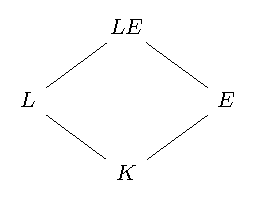
\includegraphics{lectures/6/pictures/cd_23.pdf}
		\end{center}

		Тогда мы имеем
		\[
			e = e\lr*{E/K} = [E : K] \ge [LE : L] \ge e\lr*{LE/L} = e\lr*{LE/K} = e\lr*{E/K} \cdot e\lr*{LE/E}.
		\]
		Отсюда мы получаем, что $e\lr*{LE/E} = 1$, то есть $LE/E$ неразветвлённое. 
	\end{proof}

	\begin{remark}
		Отметим, что так как поля здесь локальные, мы не говорим о сепарабельности (так как конечное расширение конечного поля сепарабельно всегда). 

		Подобные результаты можно получать и не для глобальных полей, но мы этого делать не будем. 
	\end{remark}

	На этом мы прервёмся в изучении локальных полей и перейдём к несколько другой технике, которая нам понадобится для классификации абелевых расширений поля $\Q_{p}$. 	
	 





